% The article body
% Also see main.tex for information such as authors, title, abstract, etc
% See https://www.overleaf.com/learn/ for some great resources on learning latex

\section{Introduction}

Nancy Mace, a Republican member of the U.S. House of Representatives, declares in one of her Facebook ads in 2020 that ``she's an independent thinker---while the president flaunts mask mandates, Mace requires them at her campaign events.'' Through this statement, Mace took a position that put considerable distance between herself and fellow Republican and then-president Donald Trump. Mace's decision to embrace masking is an interesting one. Perhaps Mace believed that, in spite of President Trump's opposition to mask mandates \parencite{robertson2020}, the Republican rank-and-file was much more supportive. Or perhaps Mace saw a political opportunity stemming from her gender, as we know that women candidates are thought to ``own'' issues such as healthcare and public health \parencite{shapiro1986gender} and to possess traits such as caring and compassion \parencite{huddy1993gender} that might make them better able to handle issues of public health. More broadly, we argue that a campaign's decision to mention masking in their advertisements during the height of the COVID-19 pandemic---and how they talked about masking---is quite revealing of the relative power of partisanship and gender to shape the strategic decisions that campaigns make.  

In the United States, beliefs about the appropriate response to the COVID-19 pandemic were politicized almost from its onset, resulting in differing attitudes and behaviors by partisan identification \parencite{gollust_emergence_2020,gadarian_partisanship_2021,mordecai_public_nodate}. Politicization was especially visible in regard to wearing face masks. Even as evidence emerged that COVID-19 was airborne and the Centers for Disease Control (CDC) recommended in April 2020 that all wear a cloth or fabric face covering when going out in public, President Trump remarked that the guidance was optional and that he would be unlikely to follow it \parencite{liptak2020}. Democratic presidential nominee Joe Biden, on the other hand, suggested on the campaign trail that he would implement a national mask mandate if elected and was commonly seen wearing a mask \parencite{stolberg2020}. While evidence suggests that the vast majority of the public increased its mask usage over the course of the summer of 2020, partisan gaps in the use of masks persisted, with Republicans being less likely than Democrats to report wearing them even as the overwhelming majority of Americans said they generally wore a mask when in stores or businesses \parencite{kramer_more_2020}. As Figure \ref{fig:pew} shows, the partisan gap in mask-wearing was already present by June of 2020, and it was at 10 percentage points or greater throughout that year \parencite{gramlich2022}. Perhaps unsurprisingly, then, studies have found partisan differences in excess death rates during the pandemic \parencite{wallace2022excess}. 

\begin{figure}[b] % specifier
    \caption{Pew Research Center: Partisan Divide in Frequent Mask Wearing}
    \centering % The default alignment is left.
    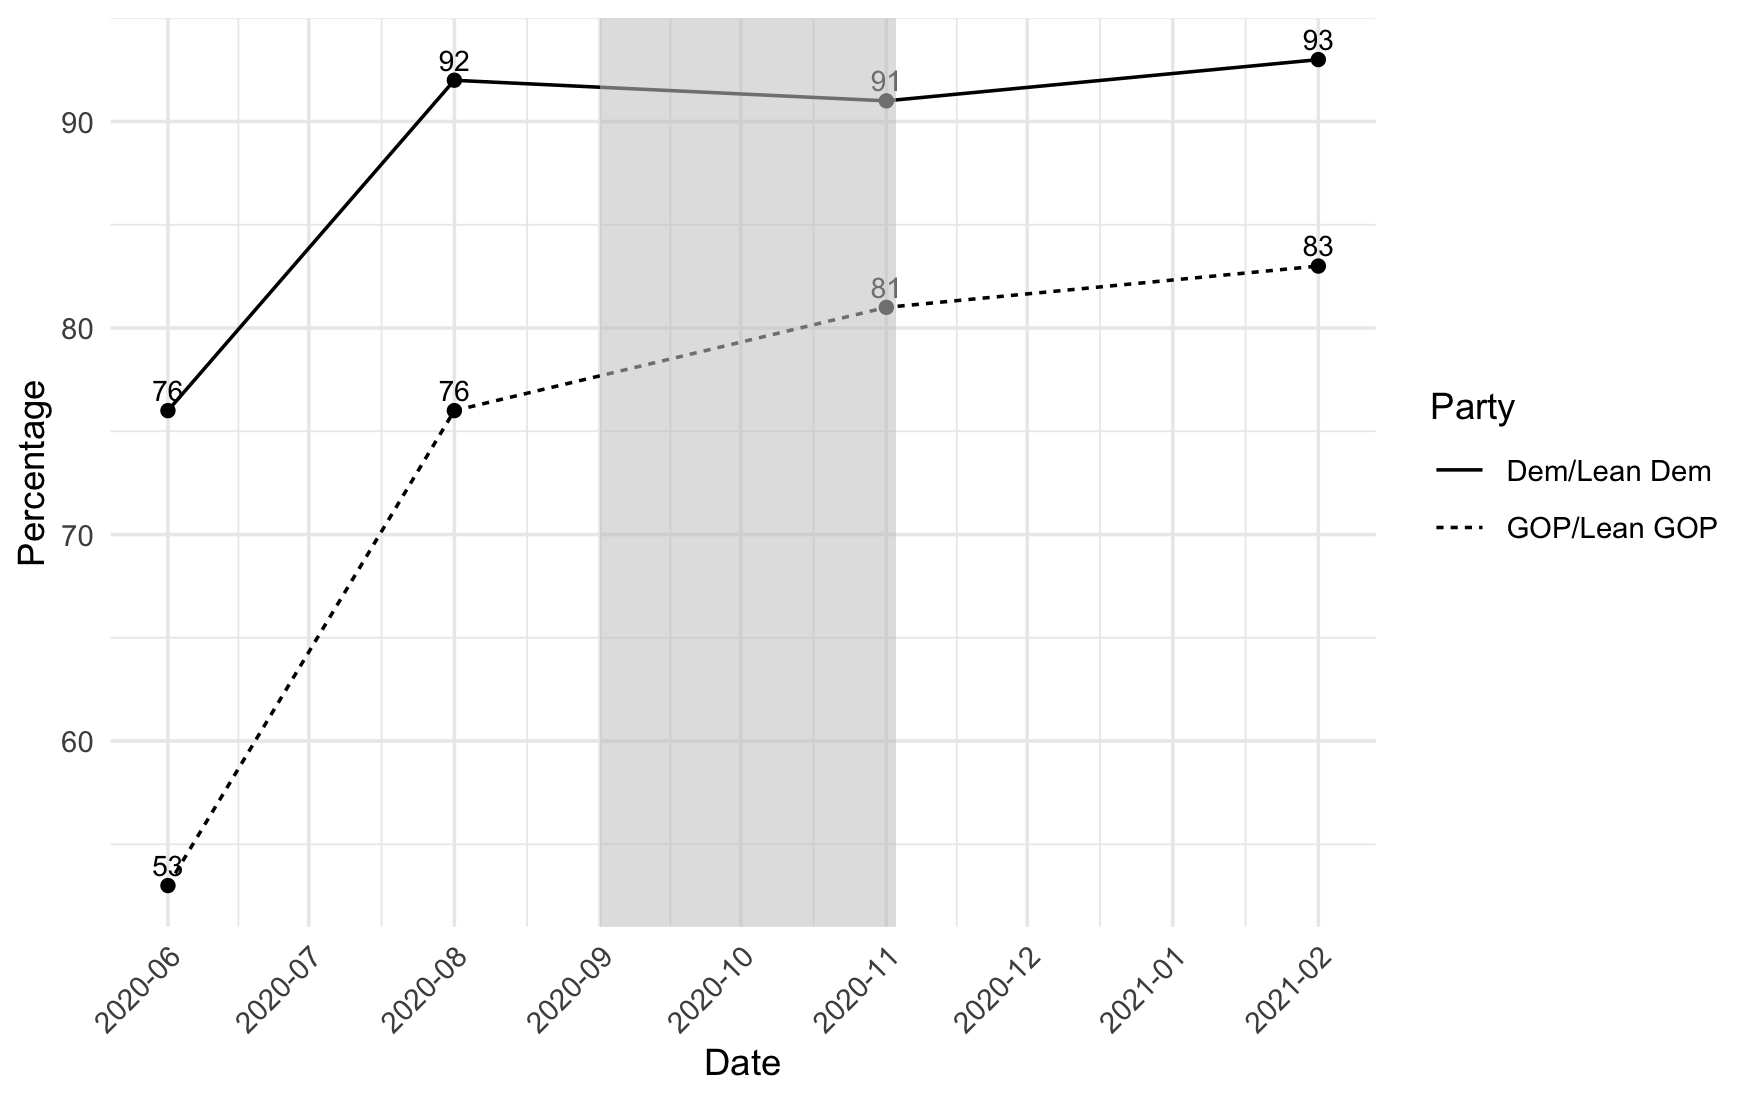
\includegraphics[width=.6\textwidth]{pew_mask.png}.
    \label{fig:pew}
    %\note{The lines indicate the percentage of U.S. adults (Democrats and Republicans) who reported that they had worn a face mask all or most of the time in stores and businesses over the past month. The shaded grey area depicts the time period covered in our analysis.}
\end{figure}

As Americans were coming to terms with the new reality of a global pandemic, the competitive 2020 election cycle was well underway, leaving candidates for federal office with decisions to make about how they might (or might not) choose to feature masks in their campaign messages. In this research, we focus on two possible predictors of the discussion and depiction of masks: the candidate's partisanship and the candidate's gender. As party polarization has contributed to decreases in citizens' trust in the government \parencite{layman2006party, fowler2015content} and thus its authority and credibility on the issue of public health, we first examine whether partisan candidates sent different or even conflicting cues on masks to the public during the crisis. Elite communication during the COVID-19 pandemic was not consistent, which hindered the public's early reaction to the crisis \parencite{green2020elusive}. We expect that partisan differences in views of masking at the national level, reflected in the different views of Donald Trump and Joe Biden, trickled down to candidates for U.S. Senate, House, and other offices, with Democrats more likely to feature masks than Republicans.  

At the same time, we investigate whether women's presence on the campaign trail could mitigate the politicization of masks as women candidates may be more willing to advocate for the use of masks in their communication with the public. Studies find that women policymakers are more likely to prioritize issues of traditional concern to women such as health care \parencite{little2001view, osborn2012women}. We also know that voters carry with them gender stereotypes, with women candidates seen as holding expertise in ``caring'' or ``compassion'' issues, such as health care \parencite{shapiro1986gender}. Thus, we may see gender differences as well in the discussion and picturing of masks.

In this research, we use automated content analysis to understand both visual and textual cues in more than 102,529 political ads on Facebook and TV. Cues, defined as small pieces of information strategically included in political messages, enable elites to subtly express their opinions \parencite{darmofal2005elite}. Visual cues have long been a crucial component of political communication \parencite{schill2012visual} and are especially important on television and social media. Politicians have incentives to use visual cues because, like verbal cues, visual cues can influence viewers' voting behavior by changing their perceptions of politicians' ideologies \parencite{dan_visual_2021}. However, scholars traditionally have overlooked visual cues in their research because of the lack of tools for systematic image or video analysis. This neglect is particularly problematic when elites decide not to prioritize an issue in their verbal discourse while employing visual symbols related to this issue to indicate their ideology or policy stances. 

Our study is distinctive in a several ways. The first is its analysis of visual depictions of masking in addition to verbal cues, as most studies of elite communication during the COVID-19 pandemic have focused on verbal cues alone (see \cite{green2020elusive, scoville2022mask, neumann2023politicizing}, with \cite{holman_masking_nodate} being one exception). The second is that we employed a state-of-the-art text analysis method -- embedding regression -- that allows us to show the context in which ``masks'' were discussed differed by candidate characteristics. The third is its focus on masking as portrayed in political advertising, which has been unexplored. Looking at advertising is important because it provides a measure of sincere campaign strategy given the large amounts that campaigns must spend on ads. Finally, our research provides  important evidence speaking to the relative influence of partisanship and gender in campaign decision-making.  

\section*{What Drives the Depiction and Mention of Masks?}
In political advertising, candidates for office regularly rely on cues, shortcuts, and symbols to signal their values, policy positions, priorities, competence, and experience \parencite{valentino_cues_2002,schmuck_effects_2017,FFR_2021,neumann2022body}. These cues are not just about the language that is being used but are often about the connection between the visual and the verbal \parencite{valentino2004impact, schmuck_effects_2017, swigger2012you}, and sometimes images are powerful on their own \parencite{FFR_2021,dan_visual_2021}. For example, candidates hoping to capitalize on their experience in the health care sector might do so by explicitly saying they are a doctor or nurse, or they might appear in a health care setting or in a doctor's lab coat. In addition, image cues in political ads can elicit emotions such as fear or enthusiasm, which can influence citizens' behavior and attitudes \parencite{brader2005striking}.

Cues in advertising can convey ideological commitments, can signal solidarity with affinity groups, and can also be used to combat racial, gendered, or other identity-based stereotypes. For example, those who want to signal support for gun rights might mention the NRA \parencite{barry_guns_2020}, or they might appear in an ad carrying a rifle or handgun even if the ad itself does not explicitly reference gun rights \parencite{FFR_2021}. In addition, candidates can stress the importance and value of specific identity groups by featuring or talking about them in their ads \parencite{connaughton_invitations_2004}. Visual cues like puppies, puffer vests, and picket fences can be deployed as a way to counter negative racial stereotypes \parencite{tesler_raphael_2020,stephens-dougan_race_2020,gillespie_race_2018,hajnal_changing_2006} while feminine visual cues, such as family and children, can be paired with masculine verbal cues to counter negative gender stereotypes \parencite{carpinella2021visual}. 

Although mask-wearing was not a political issue before the 2020 election cycle in the United States, there is every reason to believe that the decision to depict and mention masks in political ads would be strategic. First, the high salience of the pandemic meant that the decision to feature masking---one of the primary public health recommendations for combating the spread of COVID-19 at the time---was one that could not be ignored. Second, campaigns pay good money for political ads and thus make serious decisions about even minor elements of each ad's presentation. Third, political advertisements are high profile, often serving as fodder for media coverage \parencite{fowler_local_2009}, and thus the stakes are high. One Democratic ad maker explained, ``If there’s a Democrat in a Trump district who is not wearing a mask, there was strategic thought put into that, and if a Republican is wearing one in a blue-leaning seat, there’s strategy in that, too, because ads are the most expensive, well-crafted parts of the campaign'' \parencite{schneider_face_2020}.  Indeed, one ad maker did focus groups on the topic in 2020, showing a focus group pictures of candidates wearing and not wearing masks to see how people reacted \parencite{schneider_face_2020}.  In short, we expect that the decision to depict and discuss masking in political ads is strategic.

We expect the decision to depict or mention masks in political ads to fall along partisan lines.  First, cues from party leaders, Trump and Biden, may have sent a signal to voters and candidates within the party about what was appropriate masking behavior.  Second, the decision to feature masks in ads may have been a reflection of the politics of the base of each party. Evidence suggests that masking behavior is related to psychological traits, such as conflict orientation, and this relationship is mediated by support for Donald Trump and Joe Biden \parencite{young_politics_2022}. Although partisanship does not explain all variation in mask-wearing in this model, its impact is statistically significant. In addition, some citizens view wearing (or not wearing) a mask as a political statement, with a mask indicating ``submission to authoritarian rule and an emasculation of individual liberty'' \parencite{ike_face_2020}.  Thus, right-wing politicians (i.e., Republicans), who typically embrace individual liberty, may be more likely to eschew mask depictions than left-wing politicians (i.e., Democrats).

There is a third possible explanation for differences in depictions and mentions of masking across parties in 2020.  Republican candidates may have wanted to reduce discussion of masks in order to reduce the salience of the COVID-19 pandemic---and the government's sometimes bungling response. Because a Republican was in the White House at the start of the pandemic and during the 2020 election campaign, Republicans were likely to bear the brunt of the public's ire about the pandemic, and thus changing the topic to something else was likely politically smart for Republicans.  Thus, we propose our first hypothesis:  

\begin{itemize}
\item[]
\textbf{H1}: \textit{Democratic candidates are more likely to picture or mention masks than Republican candidates in their campaign ads.}
\end{itemize}

The gender of the candidate may also influence the decision to feature masks. \cite{carpinella2021visual} show that communicating femininity via visual cues is a subtle way for women candidates to address the ``double bind'' \parencite{dittmar2015navigating} that requires women candidates to display both masculine competency and feminine caring. Featuring people in masks, such as nurses and volunteers, may help women candidates to capitalize on voters' stereotypes that they are caring and compassionate. At the same time, surveys find that men are less likely to wear masks than women, and the reason for that may be notions of masculinity. Indeed, a ``toughness'' scale is a more powerful predictor of mask-wearing than is partisanship \parencite{palmer_toxic_2020}. Thus, as wearing masks themselves can help women to build an image of caring, we may find women candidates more likely to feature masks in their ads than men candidates.  Our second hypothesis is:

\begin{itemize}
\item[]
\textbf{H2}: \textit{Women candidates are more likely to picture or mention masks than men candidates in their campaign ads.}
\end{itemize}

That said, research on gender differences in political campaigning and voters' perceptions of candidates commonly notes that the effect of candidate gender is not always straightforward, as it may depend on that candidate's partisanship as well \parencite{king2003sex, huddy2002gender}. This model, referred to as a parallel processing model \parencite{schneider2016interplay}, suggests that the combination of candidate gender and party affiliation can sometimes result in something new, an effect above and beyond the effect of gender or party alone. Given the considerable empirical support for this model \parencite{schneider2016interplay}, we 
expect to find an interactive effect of party and gender in which the two identities strengthen each other, such that Democratic women are the most likely to depict or mention masks in their advertising and Republican men are the least likely to depict or mention masks.\footnote{Admittedly, the literature on candidate presentation generally finds significant partisan differences but very few gender differences in candidates' issue emphases \parencite{dolan2017candidates, sapiro2011gender}, though Strach and Sapiro (\citeyear{strach2011campaigning}) does find an interactive effect of gender and party when it comes to discussion of the attacks of September 11, 2001.}  Thus, we propose two more hypotheses:

\begin{itemize}
\item[]
\textbf{H3}: \textit{Democratic women are more likely to picture or mention masks than Democratic men, Republican women, and Republican men in their campaign ads.}

\item[]
\textbf{H4}: \textit{Republican men are less likely to picture or mention masks in their campaign ads than Republican women, Democratic men, and Democratic women.}
\end{itemize}

In addition, we explore whether Democrats and Republicans talk about masking in different ways.  Theories of campaign rhetoric, for instance, suggest that candidates emphasize frames that are more advantageous to their parties \parencite{sides2006origins}. Likewise, given that women and men candidates are believed to have different traits and issue expertise \parencite{huddy1993gender}, they may talk about masking in different ways, emphasizing those issues frames that call upon their perceived strengths. We therefore ask two research questions:

\begin{itemize}
    \item[] 
        \textbf{RQ1}: \textit{Are there differences in the ways that Democrats and Republicans speak about masking, and if so, what are those differences?}\\
    \item[]
        \textbf{RQ2}: \textit{Are there differences in the ways that men and women candidates speak about masking, and if so, what are those differences?}
 \end{itemize}

% \stepcounter{hyp}
% \setcounter{subhyp}{0}
% \begin{subhyp}
% to be added 
% \end{subhyp}

\section*{Data}

To understand whether political candidates depict and speak about mask-wearing in their campaign advertising and how, we rely on Facebook and television advertising data from all U.S. congressional candidates running in the 2020 general election collected by the Wesleyan Media Project (WMP). We focus only on candidate sponsors who placed their ads on both Facebook and television. Our final dataset contains 100,551 Facebook ads and 1,978 television ads sponsored by 350 congressional candidates between September 1, 2020, and November 3, 2020. All ads in the inference set are at the unique creative level.  For Facebook ads, uniqueness is defined as a combination of an ad's text fields. There were near-duplicates among Facebook ads due to campaigns doing A/B tests. We consider each of these near-duplicates as a unique creative because the modifications, no matter how small, were still meaningful as they were used to target different users at different times. 

The WMP collects Facebook ads through the Facebook Ad Library API which reports the sponsor who financed the ad and the dates the ad was seen. To identify political ads, WMP pulled ads through robust keyword searches that helped ensure the capture of all possible occurrences of candidate names. Using a list of candidates' Facebook page IDs, we filter the data to include only the ads sponsored by congressional candidates. The Facebook API also provides ad text data, including ad creative body, page name, ad creative link title, ad creative link caption, and ad creative description. The WMP's acquisition script allows us to download images and videos associated with the Facebook ads. 

Our television advertising data also come from the WMP, which provides access to Kantar Media/CMAG (now Vivvix/CMAG) ad-tracking data that covers broadcast television stations in all 210 media markets in the United States. The tracking data include each ad's sponsor and the time of day each ad aired. The WMP also provided the video of each ad. 

After acquiring both Facebook and television advertisements, we processed ad images and videos to obtain additional text data. We use Google's Speech-to-Text (video model) to obtain video transcription and Amazon Rekognition's \textit{DetectText} method to extract text from images. 

In addition to our key predictor variables, each candidate's party and gender, we include several control variables in our models.  One is the rurality of each congressional candidate's district or state. Early reports of COVID-19 cases were concentrated in urban areas, such as New York City, and public health advice focused on ``social distancing,'' something much easier to achieve in rural areas than in large cities.  We measure rurality using CityLab's Congressional Density Index (CDI) \parencite{montgomery2020}.\footnote{This measure starts with a calculation of households per square mile in each census tract in the country, and then each tract is placed into one of four categories, ranging from very low density to high density. An algorithm was then used to cluster each district into one of six categories.}  Because CityLab constructed their data at the district level, for U.S. Senate races, we aggregated congressional district population \parencite{us2020american} by categories and selected the CDI category with the largest population within a state. Then we recode this six-category variable into a continuous variable with 1 indicating the least rural districts and 6 the most rural districts.\footnote{Specifically, pure urban equals 1, urban-suburban mix equals 2, dense suburban equals 3, sparse suburban equals 4, Rural-suburban mix equals 5, and pure rural equals 6.} 

We use Daily Kos Elections' presidential results to obtain the share of the presidential vote obtained by Trump in 2016 either in the congressional district or state of interest \parencite{dailykos2016}.  Given that Trump was highly skeptical of masks while Biden was a proponent, support for each candidate may influence support for masking in the electorate and, in consequence, a candidate's willingness to speak about masks.

A campaign's decision to depict or mention masks may also depend on the medium, whether online or on television. Television advertising is delivered to a rather general audience and thus is designed to appeal to a wide spectrum of individuals \parencite{fowler2021political}.  Online advertising, on the other hand, is often delivered to individuals based on their characteristics and is more narrowly targeted.  We thus control for whether an ad was placed on TV (Facebook as the reference category) and whether it was a video or image ad (with image ads as the reference category). 

We drew most candidate-level data from OpenSecrets, which provides information on candidates' gender, partisanship\footnote{In the following analyses, we combined Independents with Democrats in order to examine and interpret the interaction effect between party and gender more easily. There are only four Independents that feature masks in their ads, and their stance on COVID-19 policies is aligned with Democrats.}, incumbency status and the race of interest (Senate or House).  In addition, using Roll Call's Election Guide \parencite{rollcall2020}, we constructed a four-point competitiveness variable for each race where 1 indicates safe Democratic or safe Republican, 2 indicates that a Democratic or Republican candidate is favored, 3 indicates that the race leans toward a Democrat or Republican, and 4 indicates a race that is too-close-to-call.\footnote{Ad goals and tone may influence candidates' decision to feature masks in their ads. Therefore, we used machine learning methods to identify ad goals (donate, GOTV, learn more, purchase and other), as well as ad tone (contrast, support, and attack). We included these additional controls in Tables A2, A3 and A4 of Appendix A. Note that our findings about the impact of candidate partisanship hold. We also wanted to account for the possibility that the probability of an ad featuring mask-wearing people can be influenced simply by the number of people in the ad.  Thus, we also included the number of faces as a predictor in Table A4 in Appendix A. Importantly, our central finding about the impact of partisanship holds. Note that we focused on Facebook image ads for the robustness tests in Table A4 because for the videos we did not store the number of faces when aggregating Amazon PPE detection results from the frame level to the video level in order to reduce the computational time and save storage space.} 

\section*{Methods}
To understand how candidate party, candidate gender, and their interaction affect whether candidates depict or refer to masks in their ads, we estimate the following random intercept logistic regression models stated in terms of latent linear responses:

\begin{center}
$y^{*}_{ij} = \boldsymbol{x_{ij}\beta} + \boldsymbol{u_{j}} +\epsilon_{ij}$
\end{center}
% \begin{center}
% $y^{*}_{ij} = \beta_{0} + \beta_{1}REP + \beta_{2}Female + \beta_{3}REP*Female + \beta_{4}Incumbency\_status + \beta_{5}Spend + \beta_{6}Ad\_tone +\beta_{7}Ad\_goal+\beta_{8}Pure\_rural  + \beta_{9}Competitiveness + \zeta_{j} +\epsilon_{ij}$
% \end{center}

\noindent{Our dependent variables $y_{ij}$ are binary variables indicating whether ad $i$ from candidate $j$ mentions masks or shows people wearing a mask. The vector $\boldsymbol{x_{ij}}$ are the covariates for the fixed effects, including variables of interest---candidates' gender, partisanship, the interaction of candidate gender and partisanship---as well as controls. The random intercepts $\boldsymbol{u_{j}} \sim N(0, \psi)$ are assumed to be independent and identically distributed across candidate $j$ and independent of the covariates $\boldsymbol{x_{ij}}$. The $\epsilon_{ij}$ have standard logistic distributions.

To capture whether an ad mentions masks, we search for the word ``mask'' in all text fields, including text data from Facebook API, extracted text from the images, and video transcription. We rely on Amazon ReKognition Personal Protective Equipment (PPE) detection, a deep learning model, to examine whether an ad image or video features people wearing masks.\footnote{When examining whether an ad pictures people wearing masks, we excluded ads whose media data failed to be downloaded by our script or processed by Amazon Rekognition (2.0\% of the total ads).} As shown in Figure \ref{fig:ppe}, Amazon's PPE detector can identify persons in the image and videos, the parts of a body where PPE is worn, and the types of PPE detected on body parts. In addition to the object label, the detector also returns a confidence score, which indicates the probability that a given prediction is correct. Thus, we need to specify a confidence threshold to decide whether an ad depicts a mask or not. To find the optimum threshold, we drew a stratified random sample of 300 ads from our dataset to see how the performance of the Amazon PPE detector varies with different confidence thresholds.\footnote{The strata are formed based on ad spend. We also over-sample ads that are likely to feature masks using PPE detection results (confidence score >= 90) and over-sample Facebook ads as TV ads have way higher average spending than Facebook ads. The sample consists of 125 Facebook image ads, 125 Facebook video ads, and 50 TV ads. Within each group, about half are mask ads and half are non-mask ads.} Figure \ref{fig:ppe_eval} show the evaluation results. The confidence threshold of 97 achieves the highest accuracy of 0.90 and the highest weighted average F1-score (the harmonic mean of precision and recall) of 0.90, and therefore we use it for our analysis. Finally, we construct our binary dependent variable that indicates whether an ad mentions or pictures masks.

\begin{figure}[!htbp] % specifier
    \caption{Example result of Amazon ReKognition Personal Protective Equipment detection}
    \centering % The default alignment is left.
    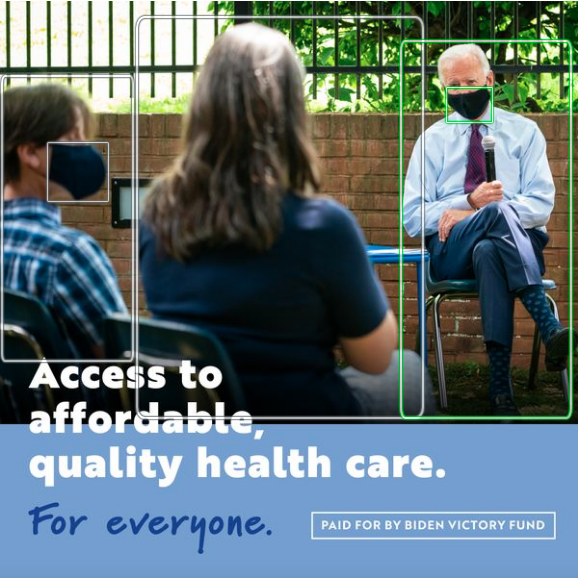
\includegraphics[scale = 0.5]{ppe_example.png}.
    \label{fig:ppe}
\end{figure}

 \begin{figure*}[!htbp] 
     \caption{Evaluation of the PPE detection of Amazon Rekognition}
    \centering
    \subfloat[Accuracy]{%
        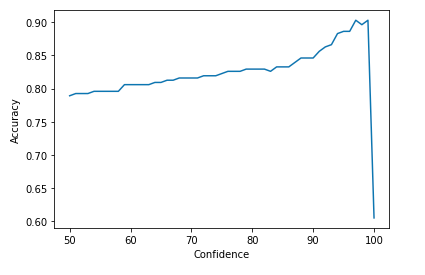
\includegraphics[width=0.5\textwidth]{ppe_accuracy.png}%
        \label{fig:ppe_eval_a}%
        }%
    \hfill%
    \subfloat[F1-score]{%
        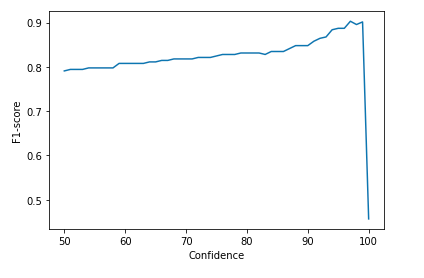
\includegraphics[width=0.5\textwidth]{ppe_f1.png}%
        \label{fig:ppe_eval_b}%
        }%
    \label{fig:ppe_eval}
\end{figure*}

In addition to analyzing whether candidates talk about masks in their ads, we are also interested in how they do so and how this relates to their party and gender. To this end, we use the \texttt{conText} embedding regression model \parencite{rodriguez2021embedding}. Traditional text analysis methods, such as WordScores \parencite{laver2003}, Fightin' Words \parencite{Monroe2008}, or Structural Topic Models \parencite{Roberts2014},\footnote{For comparison, we also include the results of Fightin' Words and a Structural Topic Model (STM) estimated on the texts that mention masks in Figures \ref{fig:fw_gender} to \ref{fig:stm_party} in Appendix B and Appendix C. These results show why Fightin' Words and Structural Topic Models are not as suited to this task. STMs can be difficult to estimate when the model becomes too complex. Moreover, in the fitted model, most of the topics are not about masks at all and mainly relate to various partisan figures. The Fightin' Words results are a little better, as the Democratic and women words in particular largely relate to masks, but there is a lot of overlap in results between those two categories.} analyze differences in the use of language across variables such as party and gender.  By contrast, \texttt{conText} seeks to answer a slightly different question: How does the context of a word---and thus its meaning---change depending on covariates? This is different from: How does the distribution of words change depending on covariates?

\texttt{conText} is tailored to target specific words. In the context of masks, this approach is appropriate because, in spite of the differences in the opinions of Democrats and Republicans, candidate from both parties commonly use the term ``mask.'' This allows us to see how Democrats and Republicans talk about masks, not just how often.

\texttt{conText} consists of two components: \texttt{a la Carte} (ALC) word embeddings \parencite{khodak2018} and a regression framework \parencite{rodriguez2021embedding}. Word embeddings \parencite{mikolov2013} are low-dimensional (i.e., 300 dimensions, as opposed to tens of thousands of token types in bag-of-words models) representations of words, where words that occur closely together during training are clustered together in the embedding space. Therefore, calculating the cosine similarity (which is effectively a non-centered Pearson correlation) between the embeddings of two words describes how closely related they are. While pre-trained word embeddings are readily available and widely used, adjusting generic pre-trained embeddings to a specific context and ensuring that even uncommon words are well-represented is difficult for small corpora. \cite{khodak2018} address this problem by mapping from pre-trained embeddings to additive embeddings for specific contexts (i.e. the averaged word embeddings of a given word's surrounding words) in what is essentially a weighted linear regression task. The parameters estimated in this regression are then used as a transformation matrix, which can be applied even to infrequent words. The newly constructed embeddings then describe the meaning of such ``focal words'' in the context of the corpus.

Most importantly, \texttt{conText} allows for hypothesis testing. It can examine whether embeddings differ significantly across levels of covariates. \cite{rodriguez2021embedding} shows that this approach even applies to focal words that occur only once and builds the regression framework \texttt{conText} on top of this intuition. In this approach, the dependent variable consists of the combined embeddings of all instances of a given focal word. The independent variables work the same way as in a traditional regression model. The regression coefficients are the estimated embeddings for all groups. The L2 norms of these coefficients can then be used similarly to traditional regression coefficient estimates, and their standard errors can be obtained via bootstrapping. We use this framework to examine whether candidates with different demographic characteristics and constituency characteristics use the term mask differently. We use the same independent variables as those in the random intercept logistic regression models. 

\section*{Results}
We first provide some descriptive analysis of mask references by candidate party and gender. We find that direct mentions of masks were rare, while masks remained an important visual cue in candidate ads. Our data show that 10,677 ads (10.4\%) in our sample featured people wearing masks, but only 396 ads (0.4\%) in our data mentioned masks verbally and 201 ads (0.2\%) did both. Moreover, the use of masks as visual cues differs by party. In terms of mask depictions, about 11.7\% of ads sponsored by Democratic candidates showed people wearing masks, while 7.2\% sponsored by Republican candidates showed people wearing masks. The difference in the use of masks as visual cues across gender is smaller; about 11.7\% of ads sponsored by women candidates and 9.2\% of ads sponsored by men candidates featured mask-wearing people. In terms of mask mentions, 0.41\% of ads sponsored by Democrats and 0.34\% by Republicans mentioned masks; 0.30\% of ads sponsored by women and 0.47\% sponsored by men mentioned masks. 

\subsection*{Party versus gender}
Table \ref{table:tab1} shows the results of our random intercept logistic regressions. All models in Table \ref{table:tab1} predict whether a mask is discussed or pictured (``featured'' hereafter) in an advertisement. In the first column, we pool Facebook and TV ads. In the second column, we show estimates from the model using only Facebook ads, and in the last column, we show estimates from the model using only television ads. 


\begin{table}[!htbp]
    \caption{Random Intercept Logistic Regression Predicting Mask Reference}
\footnotesize
    \centering
    \begin{tabular}{l*{3}{c}}
\toprule
                    &\multicolumn{1}{c}{(1)}&\multicolumn{1}{c}{(2)}&\multicolumn{1}{c}{(3)}\\
                    &\multicolumn{1}{c}{Pooled}&\multicolumn{1}{c}{FB}&\multicolumn{1}{c}{TV}\\
\midrule
Woman  &      -0.256         &      -0.330         &      -0.098         \\
                    &     (0.249)         &     (0.278)         &     (0.247)         \\
Republican     &      -0.874\sym{***}&      -0.960\sym{***}&      -0.728\sym{**} \\
                    &     (0.238)         &     (0.267)         &     (0.237)         \\
Woman $\times$ Republican&       0.122         &       0.258         &      -0.423         \\
                    &     (0.392)         &     (0.440)         &     (0.398)         \\
Rurality      &      -0.130         &      -0.116         &      -0.172         \\
                    &     (0.087)         &     (0.097)         &     (0.089)         \\
Trump vote share              &      -0.019         &      -0.020         &      -0.016         \\
                    &     (0.010)         &     (0.012)         &     (0.011)         \\
Video               &       0.761\sym{***}&       0.755\sym{***}&                     \\
                    &     (0.030)         &     (0.030)         &                     \\
Video \& image         &       1.216\sym{***}&       1.211\sym{***}&                     \\
                    &     (0.040)         &     (0.041)         &                     \\
TV                  &       1.795\sym{***}&                     &                     \\
                    &     (0.061)         &                     &                     \\
Incumbent                   &       0.518\sym{**} &       0.420         &       0.669\sym{***}\\
                    &     (0.197)         &     (0.220)         &     (0.196)         \\
Open race                   &       0.261         &       0.276         &       0.189         \\
                    &     (0.269)         &     (0.301)         &     (0.281)         \\
Senate              &      -0.390         &      -0.337         &      -0.236         \\
                    &     (0.240)         &     (0.269)         &     (0.221)         \\
Competitiveness &      -0.175\sym{*}  &      -0.193\sym{*}  &      -0.147\sym{*}  \\
                    &     (0.071)         &     (0.080)         &     (0.069)         \\
Constant            &      -1.066\sym{*}  &      -1.017         &       1.343\sym{*}  \\
                    &     (0.508)         &     (0.571)         &     (0.545)         \\
\midrule
var(\_cons[candidate\_fecid])&       2.342\sym{***}&       2.906\sym{***}&       1.176\sym{***}\\
                    &     (0.232)         &     (0.309)         &     (0.240)         \\
\midrule
Observations        &      102529         &      100551         &        1978         \\
\bottomrule
\multicolumn{4}{l}{\footnotesize Standard errors in parentheses}\\
\multicolumn{4}{l}{\footnotesize \sym{*} \(p<0.05\), \sym{**} \(p<0.01\), \sym{***} \(p<0.001\)}\\
\end{tabular}

    \label{table:tab1}
%\end{table}
%\end{center}
\end{table}

The estimates from Model (1) confirm partisan differences in the display or mention of masks, with Republican candidates significantly less likely to feature a mask than Democrats. This holds true for both Facebook ads and TV ads as shown in Model (2) and (3), and thus we have confidence in the robustness of the effect of party. According to the pooled Facebook and television model, being Republican decreases the predicted probability of featuring a mask by 0.07 using the other covariates as they were observed. Figure \ref{fig:final_gop} further shows the average marginal effect of being Republican across candidate gender on the predicted probability of featuring masks. We find that, regardless of candidate gender, the impact of being a Republican on the probability that a candidate features masks is significant and negative. For men candidates, being a Republican reduces the predicted probability of depicting a mask by 0.07, and for women candidates, being a Republican reduces the predicted probability by 0.06. Clearly, party matters for whether a mask is shown or mentioned, with Democrats significantly more likely to feature masks in an ad, and importantly, this holds even when controlling for Trump support in the candidate's district or state. Thus, our evidence supports H1. 

\begin{figure}[b] % specifier
    \caption{Average Marginal Effects of Being Republican across Gender on Pr(Masks) with 95\% CIs.}
   \centering 
   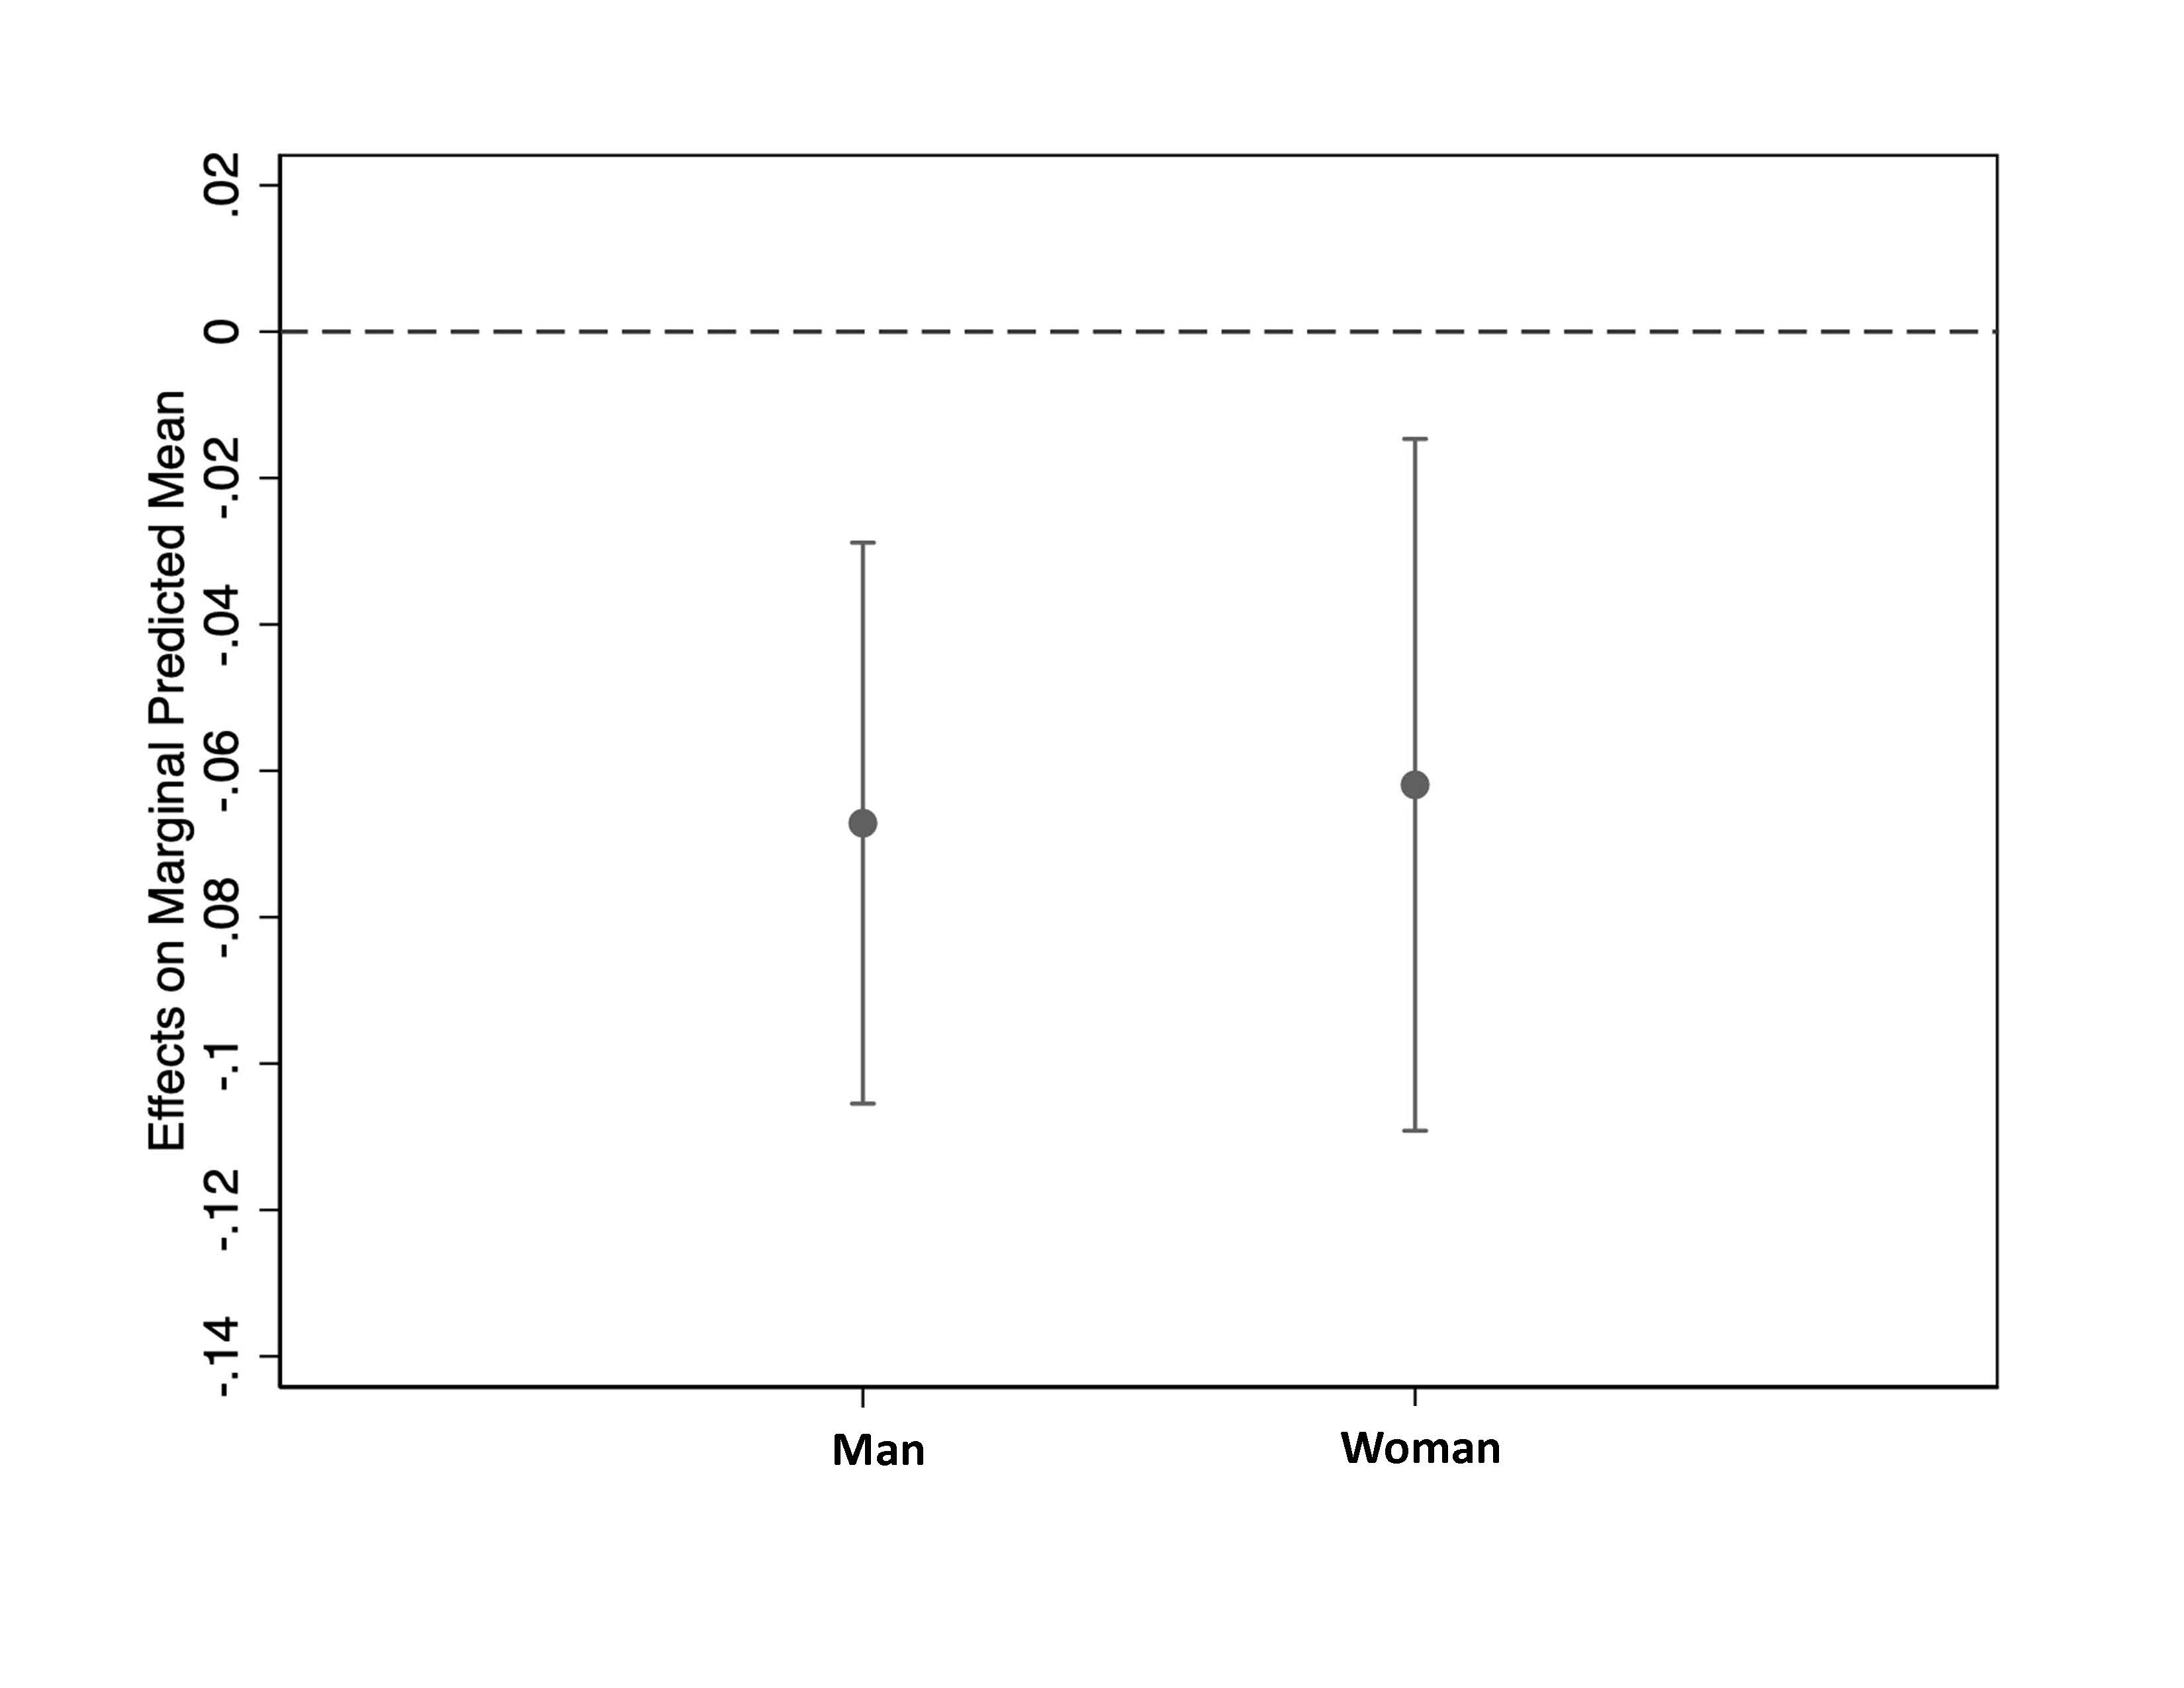
\includegraphics[width=.6\textwidth]{fig_pid_1.jpg}.
    \label{fig:final_gop}
\end{figure}

However, a candidate's gender does not affect the probability of featuring a mask. As shown in Figure \ref{fig:final_female}, we find no gender difference in candidates' decision to display or discuss masks in their ads, and this is true for both Democratic and Republican candidates.  Thus, H2 is not supported.  

\begin{figure}[b] % specifier
    \caption{Average Marginal Effects of Being a Woman across Party on Pr(Masks) with 95\% CIs.}
    \centering % The default alignment is left.
    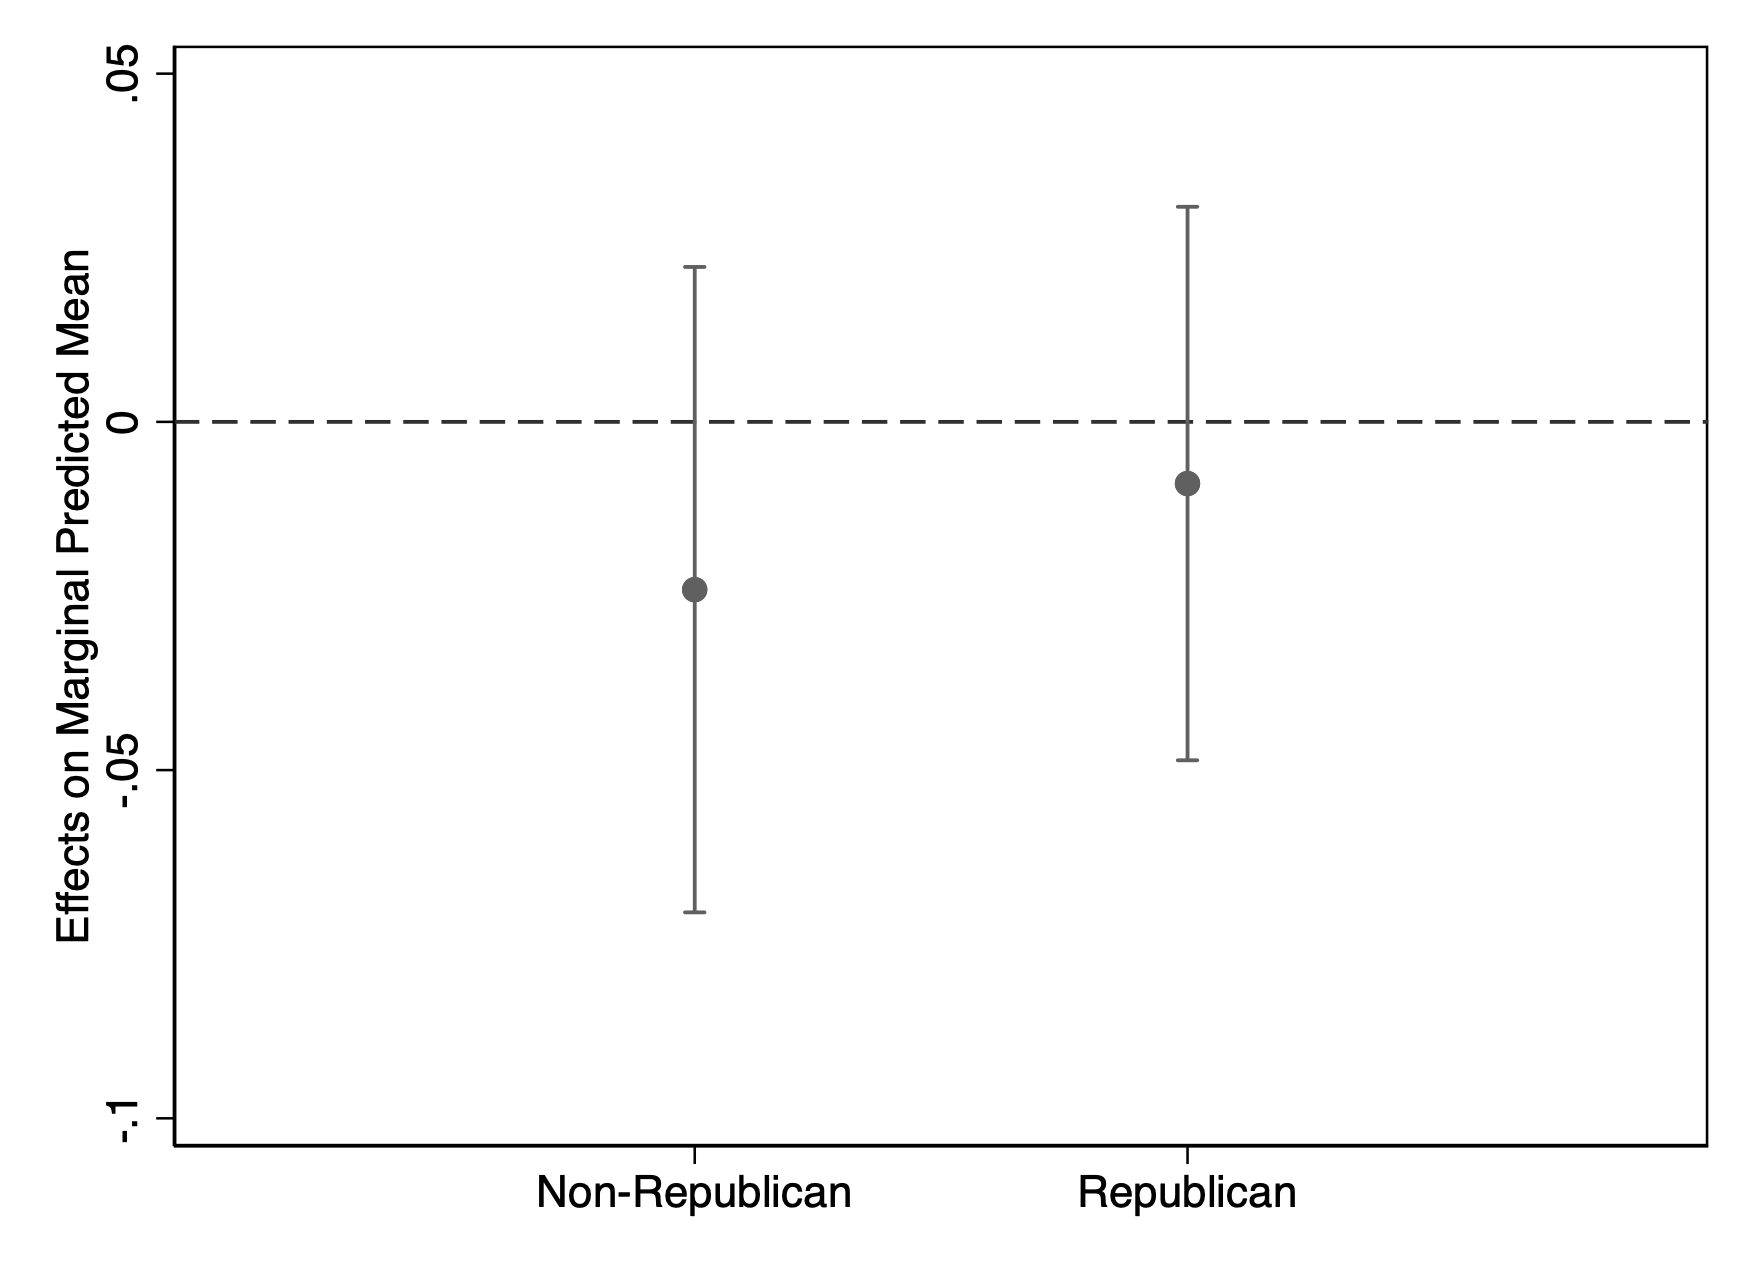
\includegraphics[width=.6\textwidth]{fig_female.png}.
    \label{fig:final_female}
\end{figure}

Our third hypothesis suggested that Democratic women were most likely to feature masks, while our fourth hypothesis suggested that Republican men were least likely to feature masks. To examine the impact of the interaction between candidates' party and gender, we calculated the average predicted probability of featuring masks for non-Republican women, non-Republican men, Republican men, and Republican women. As shown in Figure \ref{fig:final_party_gender}, although the party difference remain, there is no interactive effect of party and gender, and thus H3 and H4 are unsupported.

\begin{figure}[b] % specifier
    \caption{Average Predicted Probability of Featuring Masks with 95\% CIs.}
    \centering % The default alignment is left.
    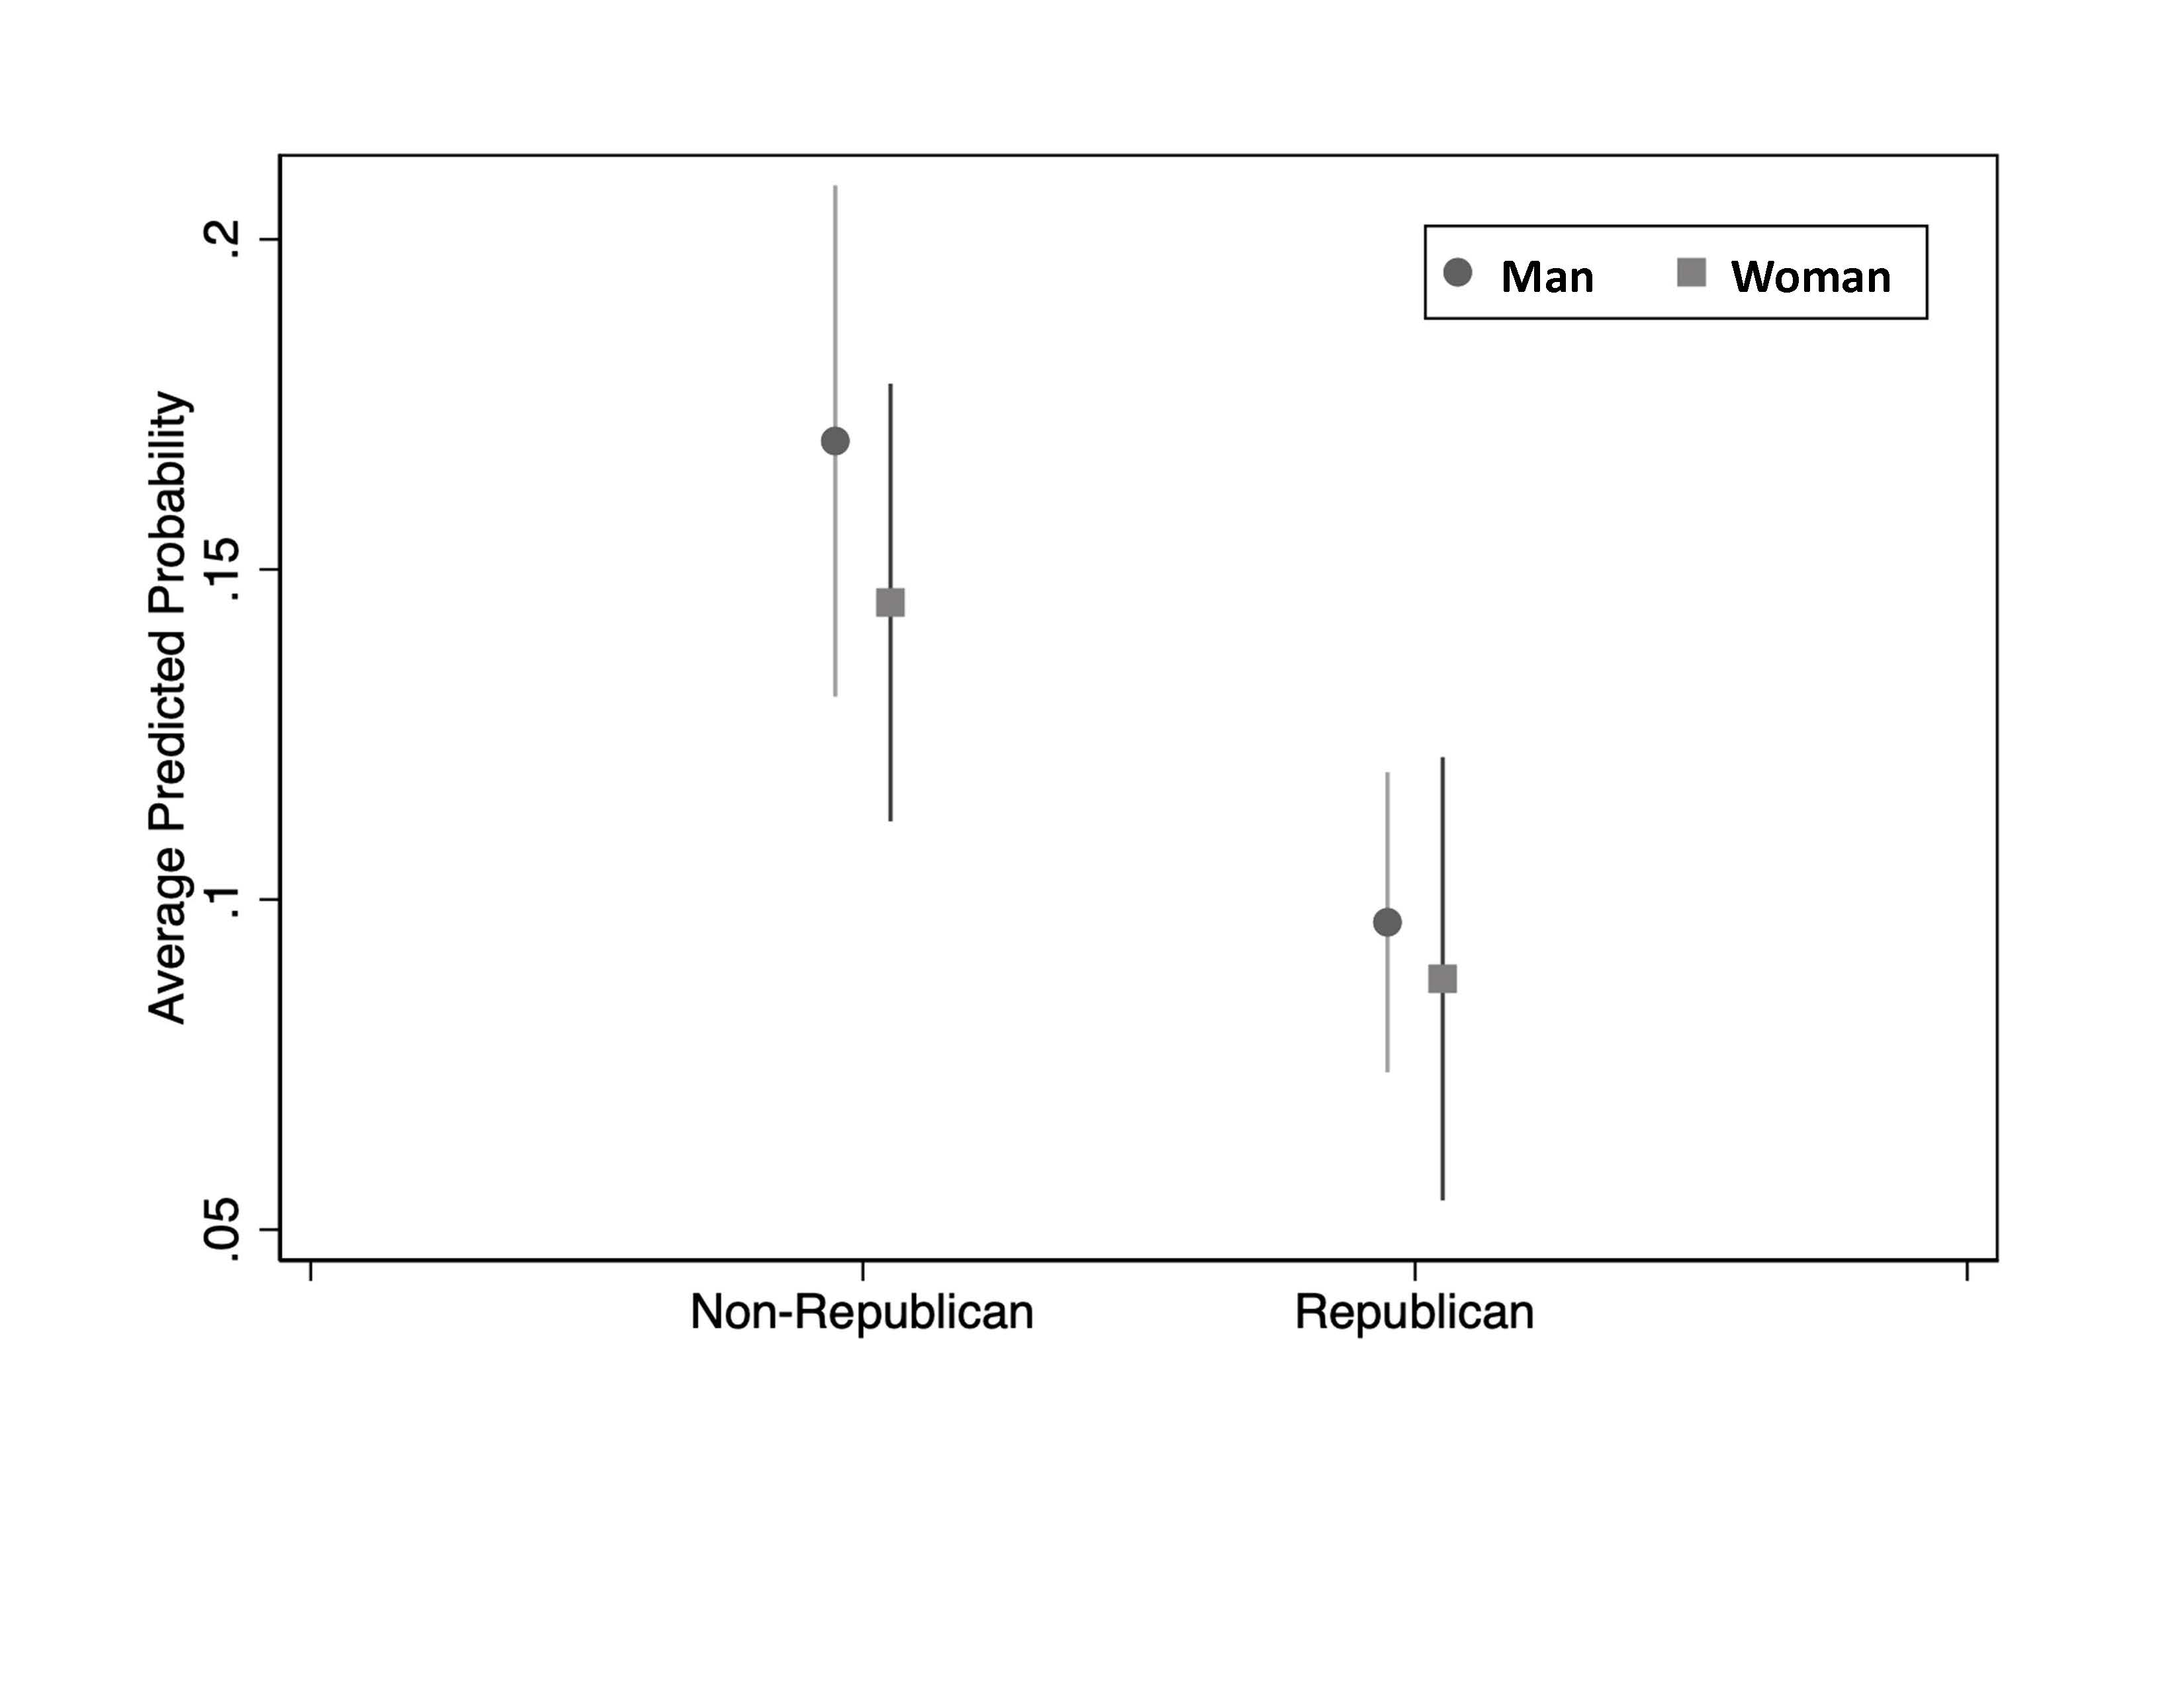
\includegraphics[width=.6\textwidth]{Fig_party_gender_1.jpg}.
    \label{fig:final_party_gender}
\end{figure}

In sum, in spite of some gender differences in the acceptance of masking among the public at large, men and women candidates feature masks in their ads at a similar frequency. Only partisanship matters when it comes to using masks as political cues. 

A couple of other control variables had a significant impact on the likelihood of an ad's featuring a mask. First, incumbents were more likely to feature a mask than challengers in the pooled and TV models. Second, the more competitive the race, the less likely a mask was featured. Third, the estimates from Model (1) show that video ads and ads with video and images are more likely to feature masks than ads without video.  Finally, television ads are more likely to feature a mask than online ads.

As a robustness check, we estimate the previous model but  separately for when masks are pictured and when masks are mentioned (results shown in Appendix A in Table A1). In the mask depictions model, the coefficient on the Republican indicator is negative and significant, just as we had hypothesized.  In the mask mentions model, the coefficient on the Republican indicator is negative and similar in magnitude to the coefficient in the depictions model, but it is not statistically significant, likely because the standard error is larger given the smaller number of ads that feature mask mentions. 

\subsection*{How do candidates speak about masks?}
Do Democratic and Republican candidates use different language when speaking about masks, and if so, how?  We examined this question through an embedding regression model. Figure \ref{fig:cr} shows the norm of the coefficients from the model. The coefficients on the Republican, woman, and Republican woman variables show the average difference across different classes, controlling for other variables. Note that magnitudes of the coefficients of embedding regressions have no natural absolute interpretation, but they can be compared relatively. In our case, the differences between Democrats and Republicans and between men and women candidates are significantly larger for our politicized focal word ``mask'' than for function words like ``and,'' ``but,'' and ``that.''  In addition, the embeddings are much larger between Republican women and other candidates. This means that, on average, the difference in the context in which the word ``mask'' is used between Republican men and Republican women is greater than the difference in the context in which the word ``mask'' is used between men and women candidates overall. 

\begin{figure}[b] % specifier
    \caption{Results of the Embedding Regressions}
    \centering % The default alignment is left.
    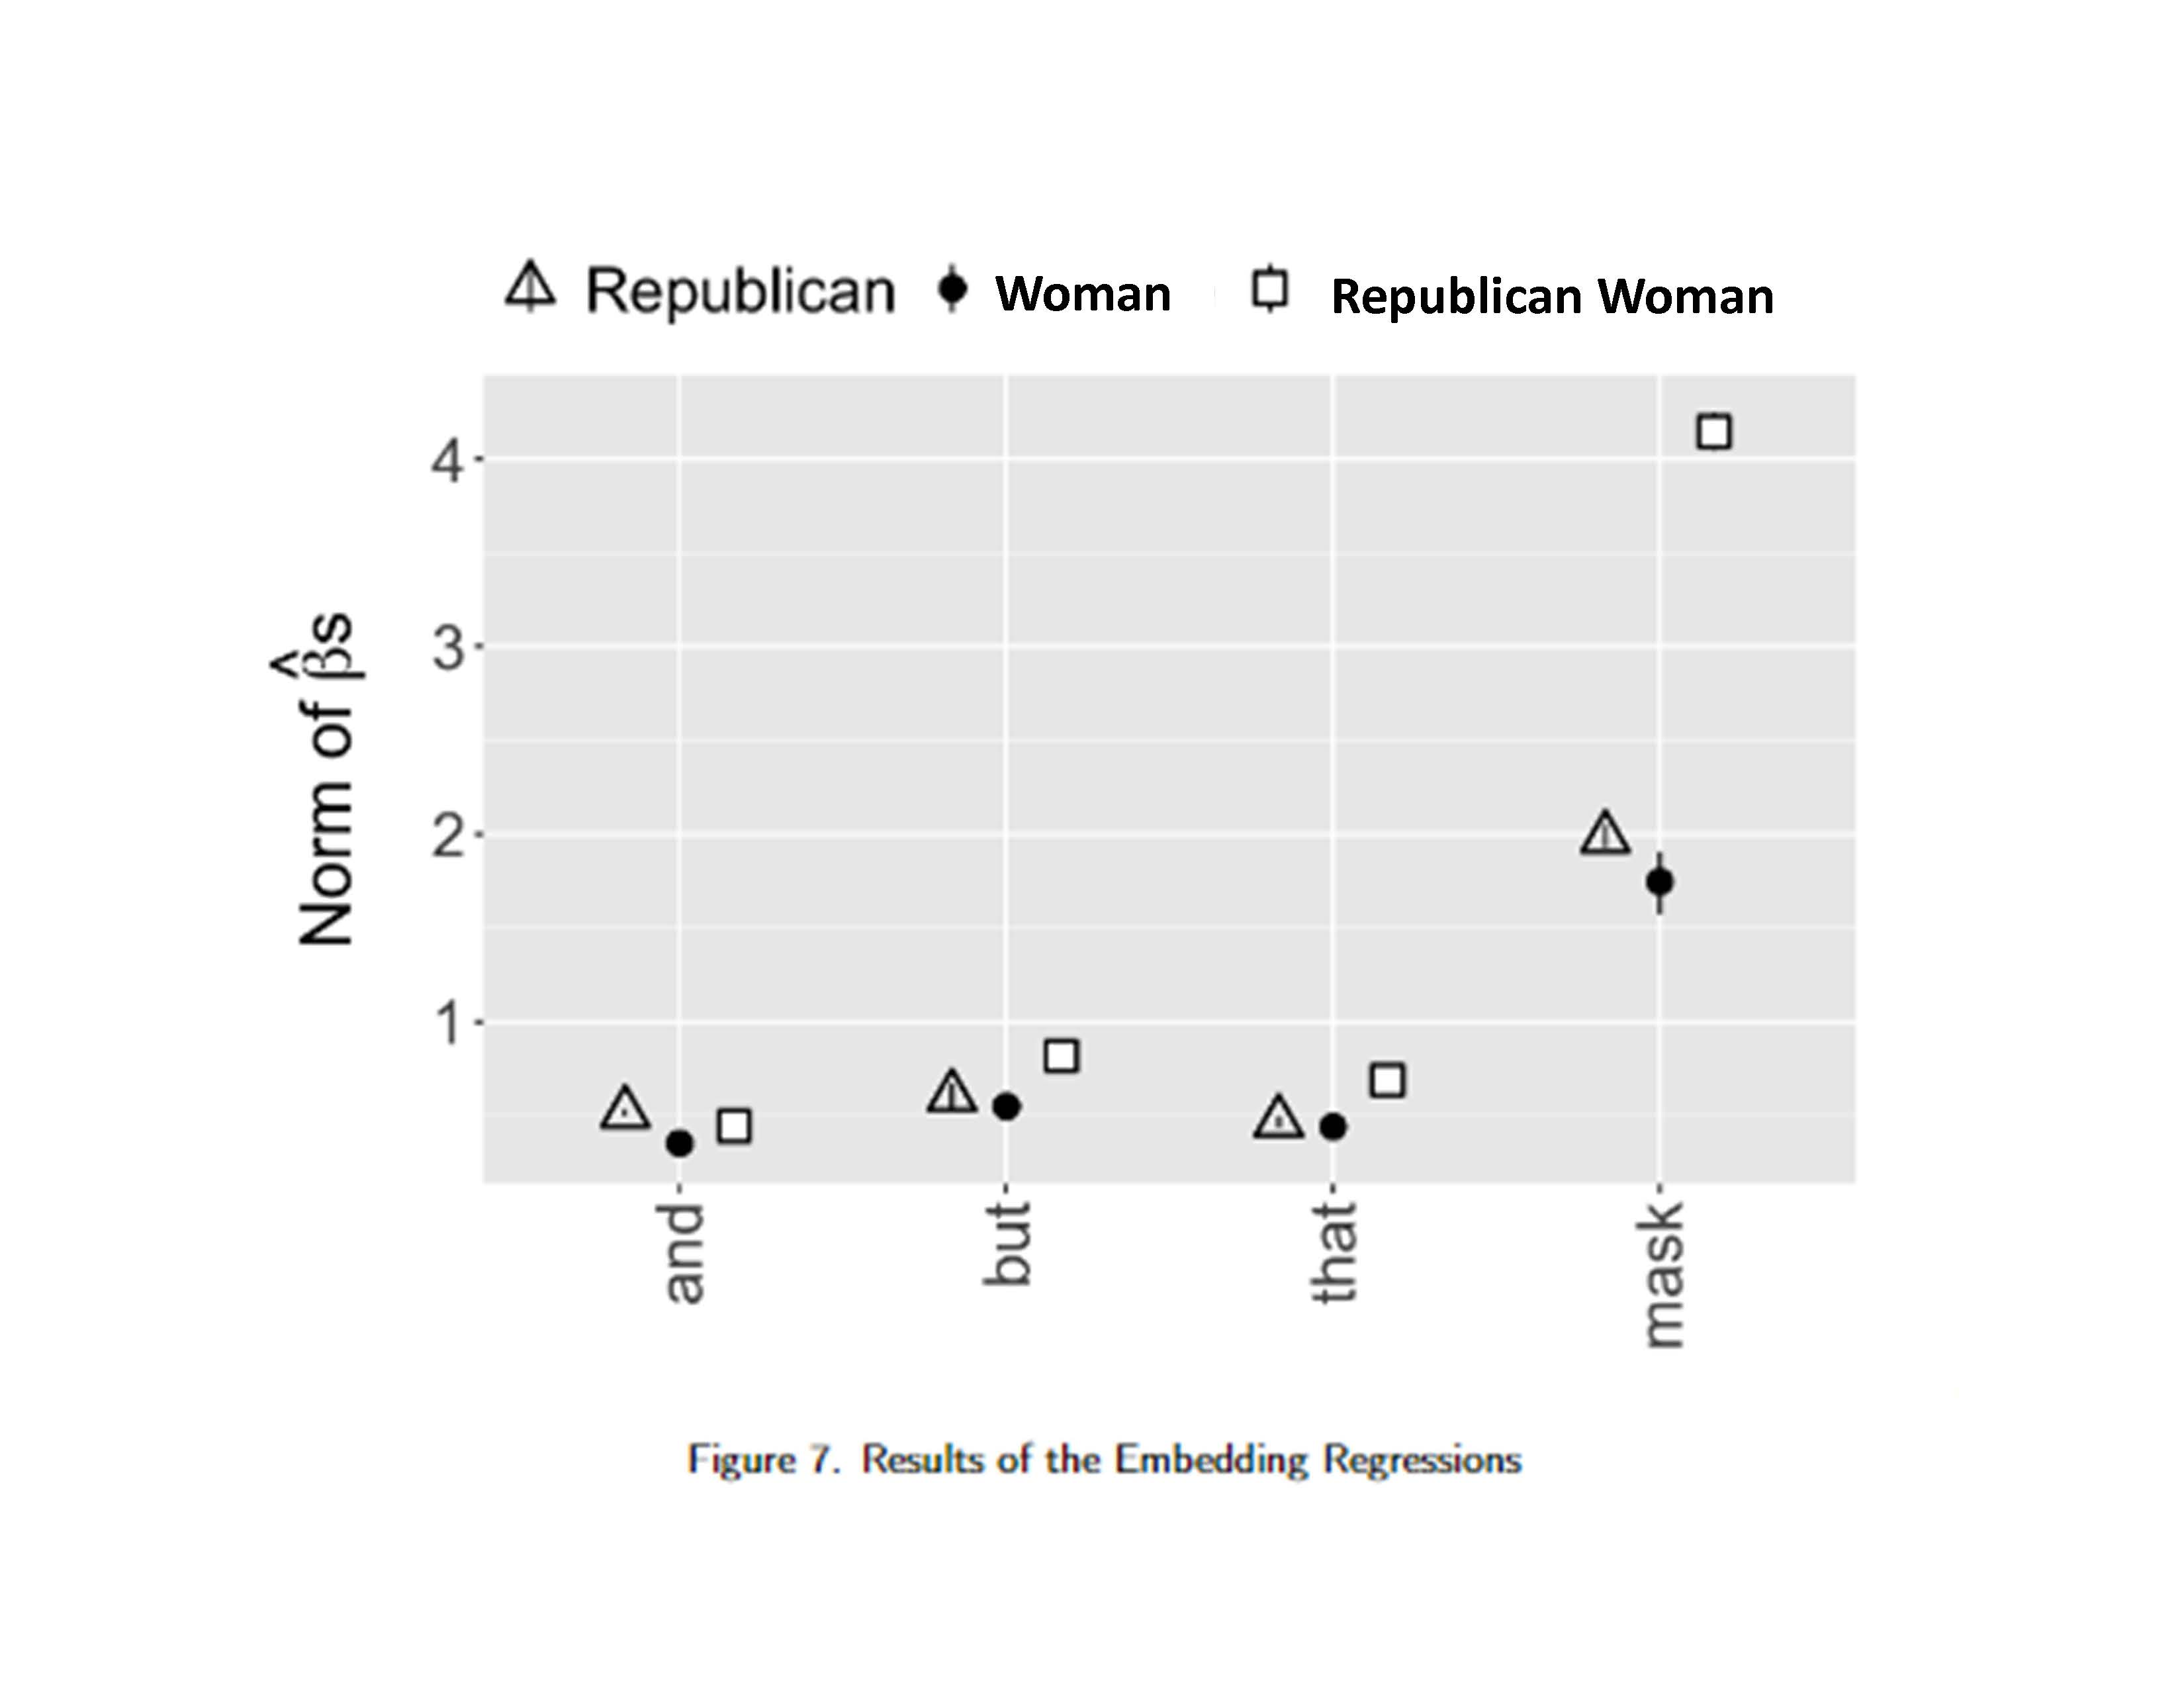
\includegraphics[width=\linewidth]{fig_cr_1.jpg}.
    \label{fig:cr}
\end{figure}

The embedding regression suggests that there are differences by party and differences by candidate gender in the way that masks are spoken about. We also wanted to be able to speak more to the nature of these differences. Thus, Table \ref{table:nn_party} shows the top 20 nearest neighbors of ``mask'' for different parties. The nearest neighbors are the vectors, that is, the embeddings of the words, closest to the estimates of how the Democrats and the Republicans use ``mask.'' There is one key difference:  the word ``health'' is in the Democratic list but not in the Republican list, suggesting that Democrats often spoke about masks in a public health context. For example, when criticizing his opponent, Sri Preston Kulkarni (D-TX) pointed out that public health experts advised that people wear masks. And Senator Mark Warner (D-VA) encouraged people to ``protect yourself and others by wearing a mask.''   

Republican candidates, however, did not convey a consistent message about the effectiveness of masks. For example, Glenn Grothman (R-WI) promised to ``fight hard to get life back to normal'' and save manufacturing ``jobs'' by making masks and medicines in Wisconsin. Though Dan Crenshaw (R-TX) mentioned that he distributed 50,000 masks for the local community in one ad, he did not do this because of the effectiveness of masks but rather provided them as a way to help people cope with mask mandates. In another ad, he told his audience to purchase a neck gaiter from his campaign website (``shop.crenshawforcongress.com''), if they ``have to wear a mask,'' so that they can go out and support ``local businesses.'' 

Table \ref{table:nn_gender} shows the top 20 nearest neighbors in ads sponsored by women and men candidates. We find that the words ``health,'' ``care,'' ``workers,'' and ``pandemic'' are close to the target word ``mask'' in the embedding of ads sponsored by women candidates, but none of these words is found among the top 20 in ads sponsored by men. This provides evidence in support of H6. Nancy Goroff (D-NY), for example, criticized her opponent Lee Zeldin (R-NY) and President Trump for ignoring scientists, not wearing masks in public, and thus putting politics ahead of citizens' ``health.'' Brynne Kennedy (D-SC) criticized her opponent for not wearing a mask to protect himself and others. Both ads implied that face masks are effective at reducing the spread of the virus. 

Do men and women candidates speak about masking differently?  Table \ref{table:nn_gender} shows the top 20 nearest neighbors in ads sponsored by women and men candidates within the Republican party. It is clear that Republican men's discourse on masks was more about purchases (``shop.crenshawforcongress.com''), ``business,'' and individuals' ability to show their support for the candidates. In contrast, Republican women were more likely to use a public health frame that points to the effectiveness of masks in preventing the spread of the virus.  One sees words such as ``wear,'' ``wearing,'' ``social,'' and ``distancing,''  none of which are found on the list for Republican men.  To provide an example, Nancy Mace (R-SC), mentioned in the introduction, stated in an ad that she required masks at her campaign events. She also expressed her worries about the virus in classrooms but insisted that parents should have the choice to send kids to school. In sum, while the word ``mask'' is used in a variety of contexts, it is more likely to be used in a public health context in ads sponsored by women than in ads sponsored by men. The gender difference within the Republican party is particularly salient.  



\begin{table}[!htbp]
%\textbf{Table 2: Top 20 Nearest Neighbors \\ for the Target Term Mask by Candidates' Party}
\caption{Top 20 Nearest Neighbors for the Target Term ``Mask'' by Candidates' Party}
    \centering
    \begin{tabular}{c|ll|c|ll}
     \hline
    \multicolumn{3}{c}{Democratic
    }&\multicolumn{3}{c}{Republican}\\ \hline
        Rank & Feature & Value & Rank & Feature & Value \\ \hline 
1 & can & 0.54 & 1 & like & 0.41 \\  
        2 & people & 0.52 & 2 & fight & 0.40 \\  
        3 & make & 0.49 & 3 & help & 0.39 \\  
        4 & help & 0.49 & 4 & shop.crenshawforcongress.com & 0.39 \\  
        5 & get & 0.49 & 5 & end & 0.38 \\  
        6 & need & 0.48 & 6 & can & 0.38 \\  
        7 & sure & 0.48 & 7 & need & 0.38 \\  
        8 & care & 0.48 & 8 & dan & 0.37 \\  
        9 & money & 0.47 & 9 & jobs & 0.37 \\  
        10 & right & 0.47 & 10 & keep & 0.37 \\  
        11 & know & 0.47 & 11 & country & 0.36 \\  
        12 & vote & 0.47 & 12 & local & 0.36 \\  
        13 & take & 0.46 & 13 & right & 0.36 \\  
        14 & time & 0.46 & 14 & protect & 0.36 \\  
        15 & health & 0.45 & 15 & make & 0.36 \\  
        16 & going & 0.45 & 16 & care & 0.35 \\  
        17 & really & 0.45 & 17 & public & 0.35 \\  
        18 & race & 0.45 & 18 & people & 0.35 \\  
        19 & end & 0.45 & 19 & back & 0.34 \\  
        20 & keep & 0.45 & 20 & work & 0.34 \\  \hline
\end{tabular}
\label{table:nn_party}
\end{table}

\begin{table}[!htbp]
    \caption{Top 20 nearest neighbors for the target term {\tt mask} by candidates' gender}
    \centering
        \begin{tabular}{l|l|l|l|l|l}
    \hline
            \multicolumn{3}{c}{Women}&\multicolumn{3}{c}{Men}\\\hline
        rank & feature & value & rank & feature & value \\\hline
        1 & workers & 0.53 & 1 & can & 0.56 \\ 
        2 & sure & 0.45 & 2 & help & 0.53 \\ 
        3 & public & 0.45 & 3 & people & 0.51 \\ 
        4 & get & 0.45 & 4 & know & 0.51 \\
        5 & make & 0.45 & 5 & really & 0.50 \\ 
        6 & health & 0.44 & 6 & back & 0.49 \\ 
        7 & care & 0.44 & 7 & need & 0.49 \\ 
        8 & pandemic & 0.44 & 8 & much & 0.48 \\ 
        9 & vote & 0.42 & 9 & take & 0.48 \\ 
        10 & people & 0.41 & 10 & right & 0.47 \\
        11 & working & 0.40 & 11 & like & 0.47 \\ 
        12 & critical & 0.40 & 12 & one & 0.47 \\ 
        13 & can & 0.39 & 13 & keep & 0.46 \\ 
        14 & use & 0.39 & 14 & give & 0.46 \\
        15 & need & 0.39 & 15 & end & 0.46 \\ 
        16 & lives & 0.38 & 16 & fight & 0.46 \\ 
        17 & work & 0.38 & 17 & make & 0.46 \\ 
        18 & businesses & 0.38 & 18 & money & 0.46 \\ 
        19 & right & 0.37 & 19 & just & 0.45 \\ 
        20 & time & 0.37 & 20 & going & 0.45 \\ \hline
    \end{tabular}
    \label{table:nn_gender}
\end{table}

\begin{table}[!htbp]
    \caption{Top 20 nearest neighbors for the target term {\tt mask} by candidates' gender within the Republican party}
    \centering
    \begin{tabular}{l|l|l|l|l|l}
    \hline
            \multicolumn{3}{c}{Republican Women}&\multicolumn{3}{c}{Republican Men}\\\hline
        Rank &Feature & Value & Rank & Feature & Value \\\hline
        1 & wear & 0.27 & 1 & shop.crenshawforcongress.com & 0.38 \\ 
        2 & place & 0.24 & 2 & people & 0.34 \\ 
        3 & mace & 0.23 & 3 & fight & 0.32 \\ 
        4 & may & 0.22 & 4 & equip & 0.32 \\ 
        5 & thinker & 0.22 & 5 & get & 0.31 \\ 
        6 & distancing & 0.21 & 6 & first & 0.30 \\ 
        7 & president & 0.20 & 7 & back & 0.29 \\ 
        8 & social & 0.19 & 8 & show & 0.29 \\ 
        9 & says & 0.19 & 9 & support & 0.29 \\ 
        10 & events & 0.19 & 10 & good & 0.28 \\ 
        11 & mandates & 0.19 & 11 & take & 0.28 \\ 
        12 & encouraged & 0.15 & 12 & make & 0.28 \\ 
        13 & right & 0.13 & 13 & strong & 0.28 \\ 
        14 & please & 0.13 & 14 & right & 0.27 \\ 
        15 & wearing & 0.13 & 15 & safe & 0.26 \\ 
        16 & battle & 0.13 & 16 & can & 0.25 \\ 
        17 & 3rd & 0.13 & 17 & jobs & 0.25 \\ 
        18 & colarusso & 0.13 & 18 & join & 0.24 \\ 
        19 & light & 0.13 & 19 & businesses & 0.24 \\ 
        20 & first & 0.12 & 20 & donation & 0.24 \\ \hline
    \end{tabular}

        
    \label{table:nn_party_gender}
\end{table}




\section*{Discussion}

Our study had several important findings.  First, candidate partisanship matters.  Democrats were significantly more likely to feature masks in their political advertisements than were Republicans during the 2020 campaigns. This finding may reflect cues from Biden and Trump, trait differences between liberals and conservatives, and a desire by Republicans to downplay the impacts of the pandemic.

Second, we found that the gender of the candidate had no impact on the featuring of a mask, and this was true within both Democratic and Republican candidates.  Clearly, a candidate's party was far more important than the candidate's gender in predicting whether an ad featured a mask. This is consistent with existing research that shows that partisan stereotypes tend to win out over gender stereotypes \parencite{hayes2011gender}.  

Third, our embedding regressions revealed there were differences in the ways that Democrats and Republicans talked about masking, differences in the way that men and women candidates talked about masking, and there were especially large differences in the way that Republican women talked about masks compared to other candidates. That is, the words surrounding the word ``mask'' were quite different for Republican women than other candidates.

That the context surrounding the word ``mask'' is different implies that candidates' party, gender, and their interaction affects how they frame masking in their communication with the public.  Of course, we should be careful with these findings given that discussions of masking, which provides the data upon which these analyses rely, are much less common than depictions of masks, especially among certain subcategories of candidates.  For example, only four ads that mention masks come from Republican women candidates. 

Finally, we presented some basic evidence in the form of a ``nearest neighbors'' analysis suggesting that Democrats were more likely than Republicans to talk about masks by using a public health frame. Democrats more commonly used words such as ``need,'' ``care,'' and ``health.'' At the same time, women candidates were more likely than men candidates to use these words suggestive of a public health frame.  Admittedly, though, it is difficult to separate partisanship from gender in these analyses given the low number of Republican women in our sample who spoke about masking.

One limitation of our study is that the ``nearest neighbors'' analysis is a blunt instrument in identifying the frames that candidates used to speak about masking.  Future research that employed human coders might be able to provide a more in-depth understanding of the way in which candidates---men and women, Republicans and Democrats---frame masking.

Another limitation is that we examine only those candidates who placed ads both on Facebook and television.  Although almost all candidates placed ads on Facebook, not all did on television.  Thus, we likely over-represented well-funded candidates in more competitive races---those who could afford to invest in television.  These are the types of candidates who are more likely to be strategic in their use of imagery, such as masks, and so if we were to included candidates who only placed ads on Facebook, we might find fewer differences across party.

\section*{Conclusion}

Our study points to an important partisan gap in the discussion and depiction of masks---and in the way that candidates talk about masking. At the same time, we demonstrate the utility of an innovative approach to generating empirical data, one that relies on a novel combination of data collection strategies.  

The partisan differences that we identified are important because, in addition to reflecting the partisan politicization of the issue at the elite level, they also likely aided in \emph{exacerbating} those partisan differences. Democratic-sponsored ads were much more likely to depict a world in which citizens, concerned about public health, wore masks, an indication of the seriousness of the COVID-19 pandemic, even if most of these ads did not discuss masking. Republican-sponsored ads, on the other hand, were less likely to feature individuals wearing masks, and rhetoric surrounding masking---while adopting various frames---was more likely to be opposed to masking.  Thus, political advertising likely helped to polarize Democrats and Republicans when it came to wearing masks.  

And this could have real-world consequences. Researchers have documented not only the effectiveness of mask-wearing in preventing COVID-19 virus transmission at the individual level but the additional benefits of mask mandates at the community level. As shown by \cite{huang_effectiveness_2022}, mask mandates reduced the number of daily cases by 23 percent at four weeks and 33 percent at six weeks. Yet such mandates are difficult to achieve when they become so politicized.  

While our substantive findings are important, our research also advances the study of computational communication. We demonstrate the use of computational techniques for the identification of both textual mentions and visual depictions of face masks, allowing us to tabulate the frequency of such mentions.  But more importantly, we establish a computational approach for demonstrating how different types of actors speak differently about masking.  We believe these techniques could be applied to discussions other topics that have become politicized, and to visual depictions of objects and symbols that have political meaning, such a bald eagle in the U.S. or a maple leaf in Canada, a country's flag, a peace sign or swastika.

With respect to political communication theory, party discussion of masking seems to support the theory of Sides (\citeyear{sides2006origins}), which suggests that, even if Democrats owned the issue of masking, there is often substantial ``issue trespassing'' by the other party. Here we saw substantial discussion of masking by Republicans, though not as much as by Democrats. Moreover, Sides suggests that the ``trespassing'' party is likely to reframe the issue, something we saw here as well, with Republicans using a variety of frames to address masking.  Interestingly, though, we did not find much evidence of Republicans using an extreme anti-masking frame: words such as ``liberty,'' ``freedom,'' and ``government'' were seldom adjacent when Republicans spoke about masks.

Our findings, of course, are the product of a particular time toward the end of the 2020 U.S. campaigns, a time before COVID-19 vaccines were available and a time during which masking overall was high and Democratic politicians were generally united in support of masking. Today, levels of masking are lower, and all states, even those with Democratic governors, have lifted mask mandates. This situation may reduce partisan differences in the depiction of masks; indeed, we may see very few ads that depict masks in the future if the current relatively low levels of COVID-19 deaths, in spite of high levels of infection, continue. But should masking become necessary again due to a new COVID-19 variant or some other pandemic, partisan differences in discussions of masking are likely to reemerge.

%\newpage
%\bibliographystyle{agsm}
%\bibliographystyle{apalike}
%\bibliographystyle{apsr}
%\bibliography{bibliography.bib}

%\newpage




